\documentclass{article}
\usepackage[]{babel}
\usepackage[IL2]{fontenc}
% \usepackage[utf8]{inputenc}
\usepackage{graphicx}
\usepackage{doi}
% \usepackage{url}
\usepackage{hyperref}
% \usepackage{enumitem}

\title{Uncovering the Ethics Behind Recommendation Systems}
\author{Serhii\;Zadorozhnyi}
\date{December 14, 2024}
\begin{document}

\maketitle
\textbf{}

\begin{abstract}
Nowadays, recommendation systems (RS) play significant part in our lives, they have many various applications such as healthcare, education, and news, they play a critical role across various digital platforms, from e-commerce to social media. They decide for us what to watch, what to buy, there to go on vacation, that may be interesting for us and more. Having a good system of recommendations is a huge benefit for any store or social media, as it can significantly enhance user engagement, drive sales, and improve customer satisfaction by providing personalized content that matches individual preferences and needs. In this paper we will talk about RS, starting with their beginning and ending up nowadays, we will discuss their impact on user experience, ethical side of RS like unfair recommendations caused by algorithmic bias, manipulation and how recommendations subtly influence our behavior and decision-making, and the transparency of algorithms, which is essential in RS to promote user trumnbv1st and clarity about origin of their recommendations, also we will discuss growin01g role of AI and machine learning in RS, highlighting both their potential benefits and risks for society. In the end, we will think about future developments in RS, which may include enhanced fairness algorithms and more user-centric personalization approaches and transparency.
\end{abstract}
% \clearpage

\section{Introduction}
Recommendation systems (RS) have now become an essential guide for decision-making on a broad spectrum of movie and book choices to restaurants and products in today's technology-merged life. Traditionally, recommendations were a result of personal insight and human interaction: one person would suggest an option to another, allowing for a nuanced exchange shaped by personal knowledge and context. However, with the inclusion of RS using AI, algorithms have been playing the lead role in compiling a personalized set of recommendations for the users.

This article summarizes the evolution of RS, starting from Elaine Rich's pioneer work on the Grundy system in 1979 \cite{F_RS} to use stereotypes for suggesting books to users. From that day forward, these systems underwent huge technological development and influenced users with their customized content. The RS become more pervasive, and with the development, critical ethical issues arise on issues such as transparency, bias, and user privacy. Furthermore, machine learning introduces potential benefits and risks, raising an overt need to approach ethical and transparent methods in system design.

In this article, we review the past, present, and future of recommendation systems; we focus on the need for interdisciplinary approaches in order to assess ethical and societal implications of algorithmic recommendations.


\section{Background}
\subsection{Classification}
Recommender systems (RS) have transformed the way digital interaction is done by providing personalized content to all. Recommender systems, when they were first evolved, were a means to recommend popular items; however, over time and with the evolution of technology, it turned into a sophisticated system with several methodologies involved in it. Within the domain of RS, there exist three basic kinds of recommendations: 
\begin{enumerate}
\item Collaborative Filtering: This recommendation form works by taking user activities  into consideration to provide shared patterns across users similar to each other. \cite{RS}
\item Content-Based Filtering: It analyzes the characteristics of items and based on that, suggests similar items to those that users already like. \cite{RS_AA_3}
\item Hybrid Systems: These systems try to combine the logics of both collaborative and content-based methods to achieve more accurate recommendations.\cite{RS}\cite{RS_AA_3}
\item Others: Beyond the primary types, additional recommendation strategies include:
    \begin{itemize}
    \item Knowledge-Based Systems: Recommend based on explicit user requirements and domain expertise.\cite{RS_AA_5}
    \item Demographic-Based Systems: Tailor suggestions using demographic information, assuming shared preferences.\cite{RS}
    \item Time-Sensitive Recommender Systems: Adjust recommendations based on temporal factors, such as seasonality or trends. \cite{RS}
    \item Location-Based Recommender Systems: Provide suggestions influenced by the user's geographical location.\cite{RS}
    \end{itemize}
\end{enumerate}
\clearpage
\begin{figure}[!h]
    \centering
    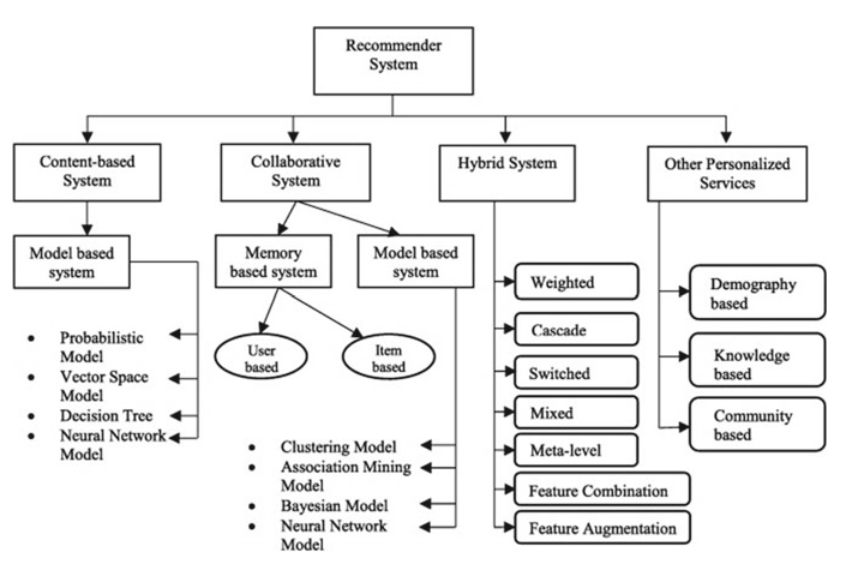
\includegraphics[width=1\textwidth]{src/RS_classification.png}
    \caption{Classification of RS \cite{RS_AA_2}}
    \label{fig:RS-Classification}
\end{figure}
% \clearpage
\subsection{First Recommendation Systems} 
The concept of recommendation systems originated in the early 1990s. Early implementations of RS were relatively simple, with most recommenders relying on popularity metrics in order to recommend items without personalized insights. For example, an e-commerce platform could show a list of "top-selling" items to every user. One of the earliest methods of personalization was collaborative filtering, which allowed recommendations to users based on commonalities among users.

\subsection{Artificial Intelligence in Recommendation Systems}

AI and machine learning turned recommendation systems from static, rule-based systems to dynamic, data-driven personalization. Techniques such as matrix factorization provide a way to extract hidden patterns in large datasets and allow for much better scalability and recommendation accuracy than ever experienced thus far, which is crucial in platforms having millions of items and users.

The evolution of RS has gone from deep learning to reinforcement learning and neural collaborative filtering, allowing insight into user behavior and contextual features such as location and time of day. Modern AI-powered RS can adapt in real time, updating recommendations based on immediate user feedback, continuously learning from the interactions to improve performance.\cite{AI_in_RS}

\subsection{Current Applications of Recommendation Systems}

RS nowadays is being deployed in a range of industries to foster engagement: from e-commerce, which suggests products based on the history of the users' browsing and purchases, to media and streaming that recommend movies, music, or news articles that best fit the taste of a user. It is also used in social media for curating feeds based on user interests, interactions, and trends.
Education and Career: Course recommendations, job openings, training by user profiles and career paths.

With AI, RS these days are more aware, responsive, and capable of complex tasks much beyond mere recommendations, which were traditional in nature. That is to say, cross-platform suggestions and real-time feedback shape digital experiences in ways unimaginable before.
\section{Ethical Challenges}
As RS increasingly affect users' experiences on many platforms, ethical concerns develop. What constitutes acceptable behavior in an ethical context regarding RS is generally subjective and often non-trivial.\cite{RS_ELI} We can, however, identify elements of RS behavior that are widely recognized as constituting ethical concerns-particularly those harming stakeholders or violating rights.\cite{IaAEC_in_RS} The following section describes some of the main ethical challenges with recommendation systems.

\subsection{Privacy}
This is a side effect of how RS works, but it creates some serious issues regarding privacy. Because recommendations are customized based on user preference, data profiles of users can be very complex and the user does not know about it. Most RS uses some forms of collaborative filtering that necessitates mass collection of data from users, including the data gathered about them from third-party sites using tracking cookies. The users often consent to vague "Terms and Conditions" that mask the actual level of data gathering, which makes it difficult for them to understand their consent.\cite{IaAEC_in_RS} Further, there are risks related to exploitation, given that breaches might lead to sensitive information leaking. Moreover, RS may infer information concerning the users from their interactions, and hence privacy concerns become much more difficult, with the user not knowing even the extent of such inferred data.\clearpage
These recommendation systems can be used to promote inappropriate or harmful material. In targeting user preferences, RS may suggest material for a user that is in line with a user's interests but is clearly inappropriate from an ethical standpoint.\cite{FB} Examples include propaganda material, racist and hate material, or materials not suitable for underage audiences. Further complications arise because the term "inappropriate content" is subjective, since it is attributed to different cultural norms and personal values...

\subsection{Personal Identity}
RS's may affect users' individual autonomy and identity. These systems generate dynamically profiles from users' data and the data of other users. Such a generation may misrepresent people's preferences and interests. This kind of misalignment can bias self-concepts of a user, creating restrictions to reach diverse content. Furthermore, there is also the risk, in the evolution of RS towards engagement-based, of creating feedback loops that reinforce given preferences with the aim of creating digital "addiction" that will exploit rather than enrich the identities of users.\cite{FB}
\subsection{Transparency}

Many recommendation algorithms are proprietary, and their internal details are kept secret to retain the competitive advantage. This limits the possibility for users to understand how their information was collected, processed, and used to arrive at specific recommendations. Informed consent of users with respect to the operation of RS's is impossible without such knowledge of the processes. Second, fairness assessment and detection of possible biases brought by algorithms are problematic when algorithms are opaque.\cite{IaAEC_in_RS}

\subsection{ Filter Bubbles}
One big ethical issue with recommendation systems is how they create filter bubbles. These systems tend to pick up on the patterns and biases in the data they're trained on, which means they often narrow down the content we see. For example, if your ratings or preferences are influenced by your friends or social circle, the system might keep showing you similar things, reinforcing those same tastes.\cite{IaAEC_in_RS}\cite{EOPIF} Over time, this creates a kind of echo chamber where you only see content that fits your existing views, while other perspectives get left out. This can be especially harmful for minority groups, who might already struggle to be seen, as it makes their voices and experiences even less visible.\cite{FB}
\clearpage
\subsection{Social Implications}

RS have the tendency to become highly socially impactful by the greater magnitude. In casting users into "filter bubbles," these systems could insulate exposure to diverse points of view, creating echo chambers. This would strangle public debate and understanding, as groups, more than ever, get to solidify their points of view without considering opposing opinions \cite{FB}. Malicious actors can use RS as a means of spreading propaganda, too. In the longer run, this might entrench division, feed polarization, and harm democratic processes.

\subsection{Inappropriate Content}
Another concern is the issues of inappropriate or, at worse, hazardous content recommendations. While the RS are designed to offer the user items based on a user's profile data, the issue is that they will still recommend items that a particular user may be interested in yet that are ethically wrong and/or socially unacceptable, they are violent, discriminatory, or not suitable for the minimum age.\cite{IaAEC_in_RS} The problem is to determine what would be considered "inappropriate" since this may significantly differ in various cultures, personal values, and norms of conduct. Further, the scale of recommendations can sometimes amplify harmful content-intentional or not-which might affect users' perception and behavior. It becomes relevant that RS are designed in such a way that they will not spread this type of content and instead foster a healthier, more responsible digital space.\cite{IaAEC_in_RS}

\section{AI and Machine Learning in Recommendation Systems}
At the heart of every recommendation system lie AI and machine learning, enabling the system to make a fairly accurate prediction of what users might like based on their behavior and preference.\cite{AI_in_RS}\cite{7956539} These systems learn from your actions, constantly getting better suggestions-often using either collaborative filtering regarding other similar users or content-based filtering, which recommends items similar to those previously favored.\cite{AI_IRS}
Deep learning and reinforcement learning are just a few of the advanced techniques allowing these systems to learn from and adapt to your dynamic preferences for more personalized experiences. But the smarter they get, the more imperative it becomes that they are transparent and fair, avoiding biases that could affect the recommendations.\cite{AI_in_RS}

\clearpage
\section{Future of Ethical Recommendation Systems}
Transparency, fairness, and user control should be the guiding principles for
ethical recommendation systems of the future. Systems that affect our choices must be
aware of biases and allow fair representation of various perspectives.\\\\
As the technology behind artificial intelligence continues to improve, recommendation systems could possibly leverage diversity in selections and thereby minimize the propensity for polarization.Users should be able to influence what they see and be clearly informed of how their data is being used.\\\\Ultimately, ethical recommendation systems should enhance the wellbeing of users, sharing accurate information while creating more inclusive online spaces.
From bias ratings-enabled news platforms to personalized social media feeds, and streaming services that recommend based on watching patterns, enhancing transparency and diversity in recommendations can have a major impact in many ways.This improvement in recommendations can help push these platforms toward online experiences that are more deliberative and inclusively oriented. 

\section{Conclusion}
In conclusion Recommendation systems have grown so big in our daily life-from what we are watching to what we're buying. While they may make our experiences more tailored and convenient, they can also raise some serious issues-for privacy, biases in recommendations can then confine people to filter bubbles where they are limited to different perspectives, and subtly manipulate their decisions. As AI and machine learning continue to improve, future recommendation systems will have to be more transparent, fair, and user-centric: give users more control, make recommendations free of bias, and develop experiences that are more balanced and inclusive. In this way, we can ensure these systems work for us, not against us, in a way that respects our autonomy and creates a healthy digital environment.
\bibliography{lit}
\bibliographystyle{IEEEtran}
\end{document}
